\section{Ejercicio 3}

El ejercicio 3 solicita implementar una red neuronal (sin POO) de dos capas densas para resolver el problema de CIFAR-10. La primera capa tiene cien neuronas y tiene la función de activación sigmoidal. La segunda capa tiene diez neuronas y activación lineal.
Se propone utilizar la función de costo MSE con regularización L2.

En primer lugar se arma el grafo computacional, y luego se programa el algoritmo de \textbf{backpropagation} para resolver el problema.
El grafo que describe este problema es el siguiente:

\begin{figure}[H]
    \centering
    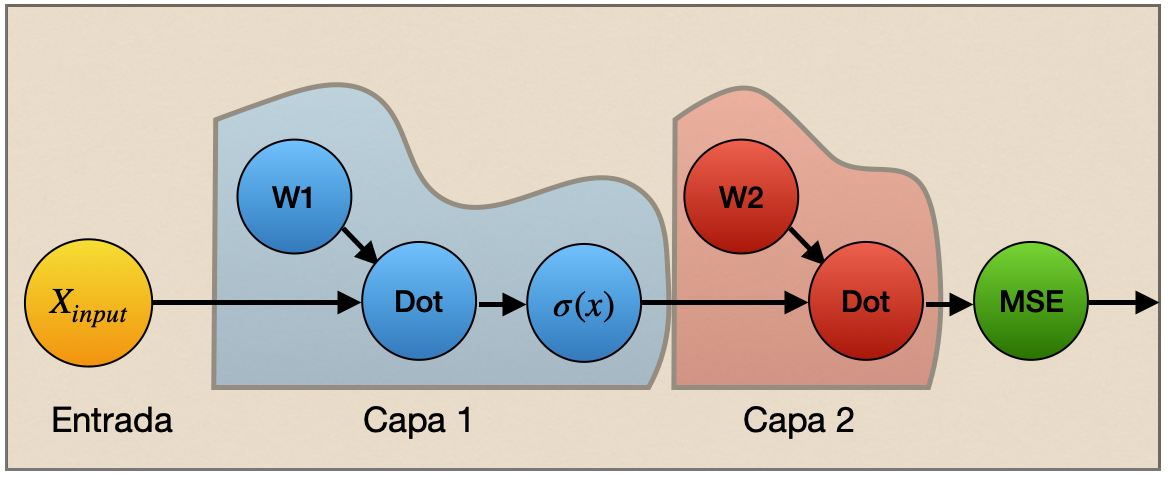
\includegraphics[height=1.5in]{image/graph3}
    \caption{Grafo computacional del problema 3}
    \label{fig:my_label}
\end{figure}

El programa comienza definiendo los hiperparámetros del problema:
\begin{verbatim}
nclases = 10            # salida
nintermedia = 100       # intermedia
batch_size = 256        # Batch size
n_epocas = 100           # Cantidad de épocas
learning_rate = 1e-7    # Learning rate
reg_lambda = 1e-3       # Coeficiente de regularización
n_train_data = 5000     # Cantidad de datos que se usarán para entrenar

\end{verbatim}
A continuación se cargan los datos de cifar y se acomodan las matrices para que puedan ser manipuladas de manera conveniente según se hizo en el Trabajo Práctico 1.
Para contribuir con la estabilidad del código se resta la media de los datos de entrenamiento tanto a los datos de \textbf{testing} como de \textbf{training} y a la diferencia se la divide por la desviación estándar de los datos de training.
Se definen matrices para expresar la salida de la red de manera que cada columna de la matriz de salida representa una clase del conjunto de datos, es decir para CIFAR-10, la cantidad de columnas de la matriz de salida es 10. Entonces, la información de a qué clase pertenece una imagen de CIFAR-10 (información almacenada en el vector \textbf{y}) se escribiría por ejemplo: 0100000000 para representar la clase 2 y 0000000001 para representar la clase 10.

Para el entrenamiento de la red neuronal, se implementó el método de \textit{Backpropagation} utilizando mini batches.
El algoritmo de \textbf{backpropagation} se realizó siguiendo el grafo computacional anteriormente presentado y llamando a las funciones de costo, de activación y gradientes correspondientes.
Además, para el cálculo de la Loss (función de costo) se aplicó la regularización L2. La función Loss se calcula haciendo:
\begin{equation*}
    Loss = \frac{1}{n} f(\hat{y}, y) + reg,
\end{equation*}
donde $n$ es el número de mini batches, $f$ es la función de costo, $\hat{y}$ es el vector de salida estimado, $y$ es el vector de salida esperado y $reg$ es la función de regularización que se calcula como:
\begin{equation*}
    reg = \sum W_1^2 + \sum W_2^2.
\end{equation*}

Realizando el algoritmo de \textit{Backpropagation} y la actualización de los pesos W, se obtienen las siguientes gráficas para el Accuracy y la Loss utilizando la función de costo MSE y con la función sigmoide como función de activación en ambas capas:

\begin{figure}[H]
     \centering
     \begin{subfigure}[b]{0.45\textwidth}
         \centering
         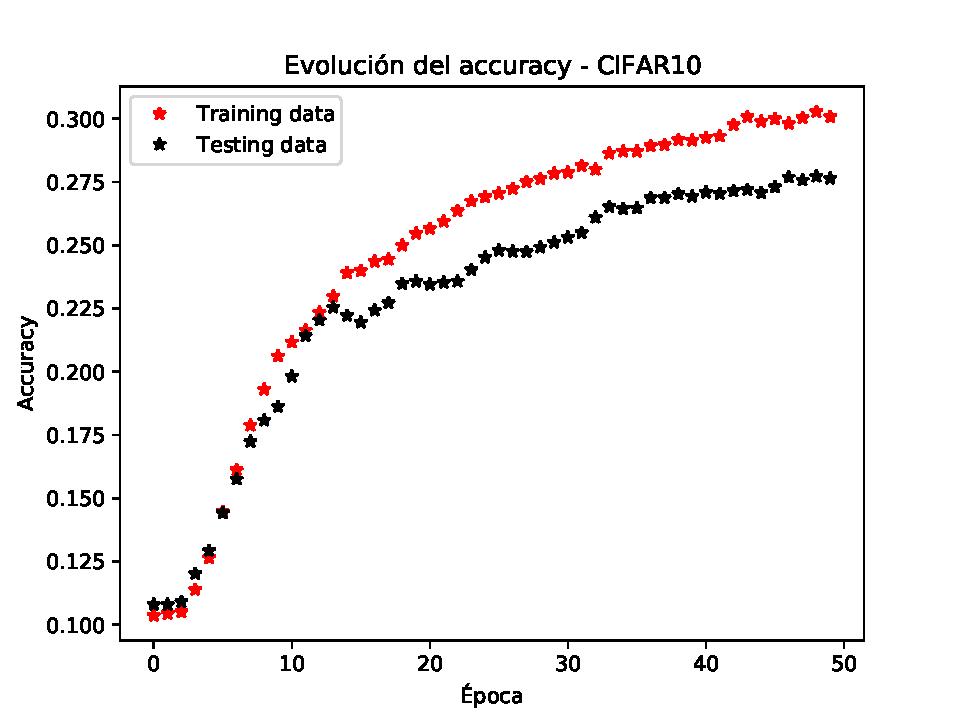
\includegraphics[width=\textwidth]{image/EJ3_Acc_SIG_LIN_MSE.pdf}
         \caption{Accuracy para el problema de CIFAR 10 aplicando Backpropagation}
         \label{fig:acc6a}
     \end{subfigure}
     \hfill
     \begin{subfigure}[b]{0.45\textwidth}
         \centering
         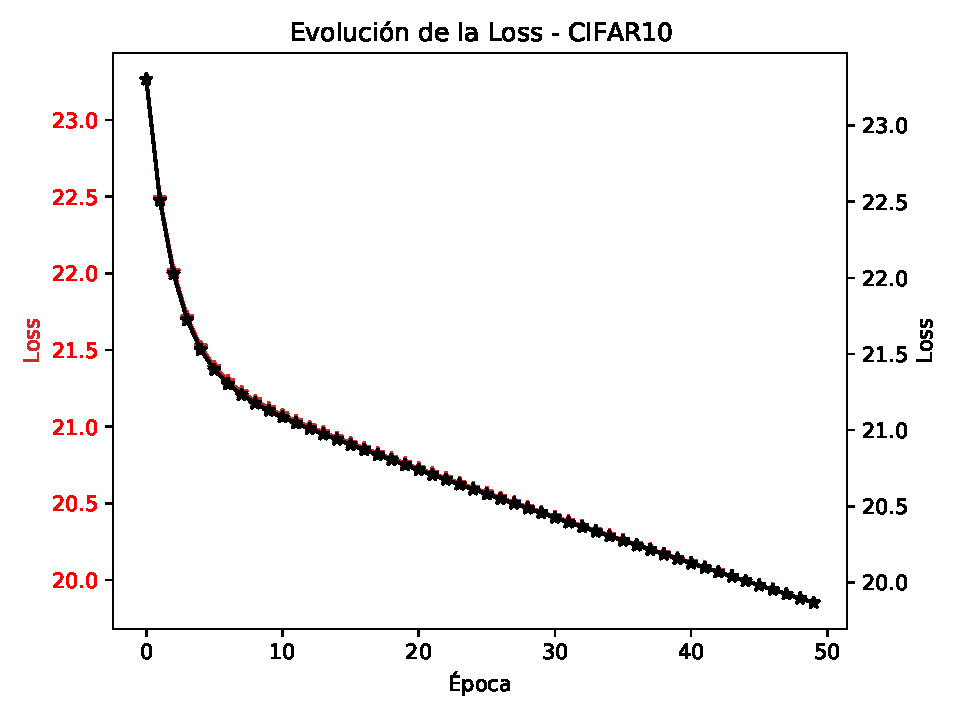
\includegraphics[width=\textwidth]{image/EJ3_Loss_SIG_LIN_MSE.pdf}
         \caption{Loss para el problema de CIFAR 10 aplicando Backpropagation}
         \label{fig:loss6a}
     \end{subfigure}
        % \caption{Resultados para la segunda arquitectura presentada para resolver el problema de la regla XOR con dos capas densas}
        % \label{fig:resu6a}
\end{figure}

Finalmente, se vio cómo cambia el accuracy cuando se utilizan respectivamente los métodos MSE (\textit{Mean Squared Error}), SVM (\textit{Support Vector Machine})y CCE (\textit{Categorical Cross Entropy}) como funciones de costo. En la siguiente figura se muestran los resultados.

\begin{figure}[H]
    \centering
    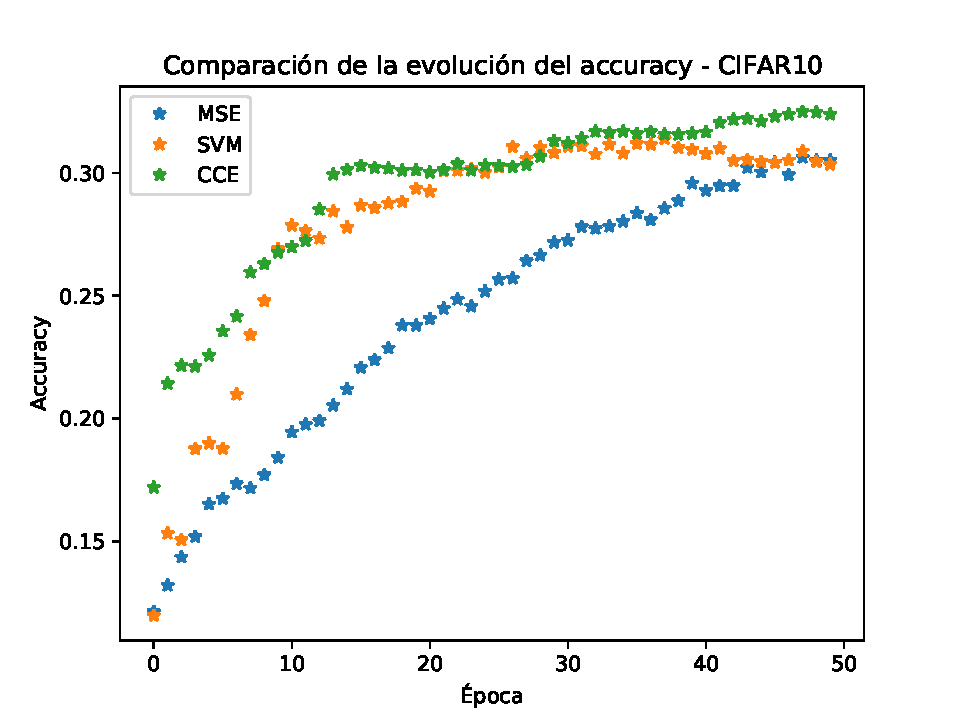
\includegraphics[height=3in]{image/EJ3comparacion2.pdf}
    \caption{Comparación de las accuracy de la red para las funciones de costo MSE, SVM y CCE.}
    \label{fig:ej3}
\end{figure}

De esta figura se ve que el método que alcanza un accuracy más alto es el CCE de SoftMax con un máximo de 38\% para 50 épocas y el método que usa MSE igualó al SVM en las 50 épocas en un valor de 30\%.

